\documentclass[conference]{IEEEtran}
\IEEEoverridecommandlockouts
% The preceding line is only needed to identify funding in the first footnote. If that is unneeded, please comment it out.
\usepackage{cite}
\usepackage{amsmath,amssymb,amsfonts}
\usepackage{algorithmic}
\usepackage{graphicx}
\usepackage{textcomp}
\usepackage{xcolor}
\usepackage[T1]{fontenc}        % Suporte para acentuação
\usepackage[utf8]{inputenc}     % Codificação de caracteres moderna (opcional em editores atuais)
\usepackage[brazil]{babel}      % Tradução geral do documento para o português
\usepackage{amsmath}
\usepackage[linesnumbered,lined,titlenumbered,ruled,noend]{algorithm2e}

%Rian
\setlength{\marginparwidth}{2cm}
\newcommand{\red}{\textcolor{red}}
\newcommand{\gray}{\textcolor{gray}}
\newcommand{\blue}{\textcolor{blue}}
\newcommand{\green}{\textcolor{olive}}
\usepackage{todonotes}
\newcommand{\addref}{\todo[color=red!40]{Add referência.}}
\newcommand{\rewrite}[1]{\todo[color=green!40]{#1}}
\newcommand{\todoin}[1]{\todo[inline]{#1}}
\newcommand{\estranho}{\todo{Estranho}}
\newcommand{\arrumar}{\todo{Arrumar}}
\newcommand{\pp}{\todo{1ª pessoa}}
\newcommand{\ac}{\todo{Arrumar cite}}
\newcommand{\veja}{\todo[color=green,fancyline]{Veja}}
%Rian

\renewcommand{\algorithmcfname}{Algoritmo}

\usepackage{listings}
\lstset{
    backgroundcolor=\color{gray!5},
    basicstyle=\small\ttfamily,
    keywordstyle=\color{blue}\bfseries,
    commentstyle=\color{green!50!black},
    stringstyle=\color{orange},
    numbers=left,
    numberstyle=\tiny\color{gray},
    frame=single,
    breaklines=true,
    captionpos=b
}

\renewcommand{\lstlistingname}{Listagem}
%\renewcommand{\lstlistlistingname}{Lista de Listagens}


\def\BibTeX{{\rm B\kern-.05em{\sc i\kern-.025em b}\kern-.08em
    T\kern-.1667em\lower.7ex\hbox{E}\kern-.125emX}}
\begin{document}

\title{BTreeFy: um \textit{framework} de \textit{Behavior Trees} para Sistemas Embarcados com Recursos Restritos}

\author{\IEEEauthorblockN{Victor R. S. de Oliveira, Bruno Nogueira, }
\IEEEauthorblockA{\textit{Instituto de Computação} - \textit{Universidade Federal de Alagoas} \\
\textit{}
Maceió, Brasil \\
\{vrso, bruno\}@ic.ufal.br}
\and
\IEEEauthorblockN{Alfredo Lima}
\IEEEauthorblockA{\textit{<Departamento ABC>} \\
\textit{<Organização XYZ>}\\
<Cidade da Organização>, <País da Organização> \\
alfredolimams@gmail.com}
\and
\IEEEauthorblockN{José Gomes, José Renilson Almeida da Silva, Rodrigo Peixoto}
\IEEEauthorblockA{\textit{Centro de Inovação Edge - Universidade Federal de Alagoas} \\
Maceió, Brasil \\
\{jose.junior, joserenilson.silva, rodrigopex\}@edge.ufal.br}
}

\maketitle

\begin{abstract}
Em aplicações de Sistemas Embarcados, o uso de máquinas de estados finitos (FSMs) é comum devido à sua facilidade inicial de uso e ampla adoção na indústria. No entanto, para a modelagem de comportamentos complexos, as FSMs apresentam limitações severas de escalabilidade e modularidade. Como alternativa, \textit{Behavior Trees} (BTs) foram concebidas para superar essas limitações. Apesar de sua popularidade em áreas como Robótica e IA, as BTs ainda são pouco exploradas em Sistemas Embarcados com restrição de recursos, devido à falta de implementações compatíveis com restrições rígidas de memória e determinismo. Para preencher esta lacuna, este trabalho apresenta o \textbf{BTreeFy}, um \textit{framework} de \textit{Behavior Tree} para Sistemas Embarcados. O \textit{framework} implementa um motor de execução iterativo sem alocação dinâmica, utiliza a representação estática \textit{Left-Child Right-Sibling} e gera código C forma automática. Para validar o \textit{framework}, conduzimos um estudo de caso de uma aplicação de rastreamento de ativos baseada no Zephyr RTOS, comparando-a com uma FSM convencional. Os resultados demonstram que as BTs promovem ganhos consideráveis de modularidade — exigindo 2,5 vezes menos linhas de código para adição de uma funcionalidade —, enquanto impõem custos de memória relativamente baixos (\textasciitilde 1 KB de Flash) e mantêm latências de execução totalmente compatíveis (na faixa de dezenas de microssegundos) para a vasta maioria das aplicações de tempo-real.
\end{abstract}

\begin{IEEEkeywords}
Sistemas Embarcados, \textit{Behavior Trees}, C, \textit{framework}, \textit{left-child right-sibling}
\end{IEEEkeywords}

\section{Introdução}

A modelagem de comportamento em Sistemas Embarcados adota tradicionalmente o formalismo de Máquinas de Estados Finitos (FSMs) como o método mais comum de controle. O uso desse modelo pode ser associado à sua facilidade inicial de compreensão, ao seu histórico de aplicação na indústria e à sua presença nos currículos de engenharia e de ciência da computação. Como o projeto de firmware muitas vezes requer a gestão de estados e interrupções, as FSMs costumam surgir como uma escolha natural para a modelagem da lógica de controle. Entretanto, à medida que a complexidade dos sistemas embarcados aumenta, as características arquitetônicas das FSMs podem apresentar desafios de escalabilidade e manutenção. O modelo de Máquina de Estados é basicamente um grafo dirigido onde os nós são os estados e as arestas são as transições, as quais são responsáveis por conectar os estados entre si e normalmente representam condições ou a ocorrência de eventos em um sistema. Devido a essa topologia, a adição ou remoção de estados exige a reavaliação de um número potencialmente grande de transições e estados internos do modelo. FSMs com muitos estados e transições são difíceis de modificar, o que impõe barreiras severas à escalabilidade \cite{biggar_expressiveness_2021}.  
Além do impacto na manutenibilidade, podem surgir desafios do ponto de vista de modularidade. Como as transições frequentemente dependem dos estados e de suas variáveis internas, o uso de extensões hierárquicas (HFSMs) pode atenuar essa deficiência, mas não a soluciona por completo. Consequentemente, o reúso de lógicas de controle entre diferentes projetos ou módulos torna-se uma tarefa mais complexa e propensa a erros, motivando a investigação de abordagens arquitetônicas alternativas para a orquestração de execução em firmware \cite{iovino_comparison_2025}.

Um formalismo que tem ganhado destaque para modelagem de comportamento é a \textit{Behavior Tree} (BT). Originalmente concebidas para superar as limitações das FSMs na inteligência artificial de jogos (oferecendo maior modularidade e reatividade), as BTs tornaram-se populares não apenas em jogos, mas também em robótica, sistemas autônomos e controle industrial \cite{sidorenko_towards_2024}. Apesar desse sucesso, sua aplicação em sistemas embarcados tem sido pouco investigada. Contudo, sua natureza baseada em eventos, operando através da propagação de \textit{ticks}, alinha-se de forma natural à dinâmica desses sistemas, oferecendo abstrações modulares e seguras para lidar com fluxos de controle complexos.

Aplicações em Sistemas Embarcados com Recursos Restritos são tipicamente compostas por microcontroladores operando com severas limitações de memória (frequentemente na casa de dezenas a poucas centenas de \textit{kilobytes} de RAM e Flash), ausência de unidade de gerenciamento de memória (MMU) e a necessidade estrita de determinismo temporal.
Tais sistemas operam tipicamente em abordagens \textit{bare-metal} ou são orquestrados por Sistemas Operacionais de Tempo Real (RTOS) leves. Sob essas restrições, a arquitetura de software deve evitar a alocação dinâmica de memória (\texttt{malloc}/\texttt{free} ou \texttt{new}/\texttt{delete}), prevenindo a fragmentação da memória e a imprevisibilidade do tempo de execução, priorizando estratégias de alocação estática para garantir tempos de resposta delimitados.

Um dos principais motivos pelos quais BTs têm sido pouco exploradas na área de Sistemas Embarcados com Recursos Restritos é a falta de bibliotecas ou \textit{frameworks} adaptados ao ferramental e às rigorosas restrições arquiteturais desse ambiente. O levantamento de Iovino \textit{et al.} \cite{iovino_survey_2022} listou diversas bibliotecas de BTs disponíveis, implementadas em linguagens como Python, Java, C\#, C++ e JavaScript. Embora o C++ possa ser utilizado em sistemas embarcados, as implementações tradicionais de BTs abusam frequentemente de alocação dinâmica, concorrência complexa e ponteiros inteligentes (\textit{smart pointers}), o que fere os princípios de determinismo requeridos para esse nicho. Além disso, os ambientes de desenvolvimento para microcontroladores restritos tipicamente não oferecem suporte — ou vedam explicitamente, por meio de diretrizes de segurança e determinismo como MISRA C++ e ISO 26262 — a recursos amplamente utilizados nas implementações convencionais de BTs em C++, como alocação dinâmica de memória, biblioteca padrão de \textit{templates} (STL), tratamento de exceções e informações de tipo em tempo de execução (RTTI). As implementações convencionais de BTs constroem-se justamente sobre esses recursos do C++ moderno, tornando a sua integração direta em plataformas embarcadas restritas técnica e arquiteturalmente impeditiva.

Com o intuito de preencher essa lacuna, este trabalho propõe um \textit{framework} de \textit{Behavior Trees} para Sistemas Embarcados com Recursos Restritos, chamado \textbf{BTreeFy}. O desenvolvimento deste \textit{framework} tem por objetivo atender às demandas específicas deste nicho, garantindo previsibilidade de tempo real e baixo consumo de recursos computacionais. Desta maneira, as principais contribuições deste trabalho são: (i) uma estratégia de implementação através de motor de execução iterativo e representação \textit{left-child right-sibling} dos nós da \textit{Behavior Tree}; (ii) um \textit{framework} funcional desenvolvido na linguagem ANSI C, livre de alocação dinâmica e dependências de bibliotecas de terceiros, além de uma ferramenta utilitária para geração de código automático a partir do editor \textit{Groot 2}; (iii) um estudo de caso para validação da aplicabilidade de \textit{Behavior Trees} em aplicações de sistemas embarcados.

% 1. Uma adaptação para utilização de BTs em sistemas embarcados
% 2. Framework (API + geração de código)
% 3. Estudo de caso

\section{Fundamentos em Behavior Trees}

\textit{Behavior Trees} são um formalismo de controle utilizado para descrever tarefas em agentes ou sistemas e foram desenvolvidos com o intuito de superar algumas limitações das Máquinas de Estados Finitos com relação a reatividade, modularidade e legibilidade. Conceitualmente, uma \textit{Behavior Tree} é uma árvore cujos nós intermediários são chamados de \textit{nós de controle de fluxo} e os nós folha são chamados de \textit{nós de execução}.
Os \textit{nós de controle de fluxo} têm a função de implementar uma política que determina qual o próximo nó a ser executado, enquanto os \textit{nós de execução} implementam verificações de condições ou ações do sistema.
Quando uma condição ou ação é executada, o nó pode retornar três valores de \textit{status} possíveis: \textit{Failure}, \textit{Success} ou \textit{Running}. Os valores de \textit{Failure} e \textit{Success} indicam, respectivamente, uma falha ou um sucesso na execução do nó, enquanto o valor \textit{Running} indica que o nó ainda não concluiu sua execução e será reexecutado em seguida.
É imperativo destacar que, em qualquer nó de controle de fluxo, a ordem de avaliação e execução dos nós filhos ocorre \textbf{sempre} da esquerda para a direita. Essa restrição introduz naturalmente uma noção de prioridade no modelo, onde ramificações mais à esquerda possuem precedência de verificação sobre as ramificações à direita. Essa característica é fundamental, pois motiva fortemente o uso da representação de árvores estruturadas como \textit{Left-Child Right-Sibling} (LCRS), que será discutida adiante.

\subsection{Nós de controle de fluxo}

Considerando a formulação clássica apresentada em \cite{colledanchise_behavior_2018}, uma \textit{Behavior Tree} pode possuir os seguintes tipos de \textit{nós de controle de fluxo}: \textit{Sequence}, \textit{Fallback}, \textit{Parallel} e \textit{Decorator}.
Cada um desses nós, quando executado, realiza a execução dos seus respectivos filhos (ou do filho, no caso do \textit{Decorator}).

%Em sua formulação clássica, de acordo com \ref{colledanchise_behavior_2018}, os \textit{nós de controle de fluxo} básicos em uma \textit{Behavior Tree} são: \textit{Sequence}, \textit{Fallback} e \textit{Parallel}. 

Quando um nó \textit{Sequence} é executado, ele executa seus respectivos filhos, em sequência da esquerda para a direita, até que um deles retorne \textit{Failure} ou \textit{Running}, em que, nesta situação, a execução retorna o valor resultante ao seu respectivo nó pai. Assim, o nó \textit{Sequence} apenas retorna \textit{Success} se todos os seus filhos retornarem \textit{Success}. 

\red{Qual o desenho de representação do nó?}

De forma semelhante, o nó \textit{Fallback}, quando executado, realiza a execução dos seus filhos, da esquerda para a direita, até que um deles retorne \textit{Success} ou \textit{Running}, e então, sua execução retorna para seu respectivo nó pai. Assim, o nó \textit{Fallback} só retorna \textit{Failure} se todos os seus filhos também retornarem \textit{Failure}.

\red{Qual o desenho de representação do nó?}

O nó \textit{Parallel}, por sua vez, também executa seus nós filhos da esquerda para a direita, mas sua execução só resulta em \textit{Success} se \texttt{M} nós filhos retornarem \textit{Success}. Caso contrário, retorna \textit{Failure}.

\red{Qual o desenho de representação do nó?}

Por fim, o nó \textit{Decorator} é um tipo de nó que aceita apenas um filho. O comportamento de um nó \textit{Decorator} é definido através de uma regra personalizada pelo usuário. No entanto, existem comportamentos comuns pré-definidos normalmente encontrados em implementações de \textit{Behavior Tree} como o \textit{Decorator} de \textit{inversão}, que inverte o valor retornado de um nó filho de \textit{Failure} para \textit{Sucesso} ou \textit{vice-versa}, além de outros comportamentos como o \textit{Decorator} de execução \textit{máxima de N tentativas} ou \textit{repetição enquanto Success}, cujos nomes são autoexplicativos.

\red{Qual o desenho de representação do nó?}

\subsection{Nós de execução}

Os nós que não possuem filhos ou folhas de uma árvore são considerados nós de execução em uma \textit{Behavior Tree}. Esses nós podem representar dois tipos de execução: \textit{condição} ou \textit{ação}. A diferença entre esses tipos de nós é apenas conceitual. O \textit{nó de condição} indica a execução de verificação de uma condição, e sua execução pode retornar apenas os valores \textit{Failure} ou \textit{Success}. Já o \textit{nó de ação} indica a execução de uma ação ou tarefa e sua execução pode retornar \textit{Failure}, \textit{Success} ou \textit{Running}.

\red{Qual o desenho de representação dos nós?}

\subsection{Execução de uma Behavior Tree}

A execução de uma \textit{Behavior Tree} é baseada na propagação de um sinal comumente chamado \textit{tick}, que determina a execução de um nó. A propagação do \textit{tick} é iniciada a partir da raiz da árvore e percorre todos os nós da árvore seguindo a ordem do nó filho mais à esquerda, até que um nó folha seja atingido. Quando um nó folha é atingido, seu valor de \textit{status} é retornado ao seu respectivo nó pai. Neste momento, o nó pai executa sua função de política para determinar qual o próximo nó a ser executado. A depender desta decisão, o próximo nó a ser executado pode ser um nó filho à direita, ou a execução pode retornar para o nó acima, em direção à raiz da árvore. Este processo de propagação do \textit{tick} pelos nós da árvore permanece até que o nó raiz seja avaliado e não haja mais nós a serem executados.

Vale ressaltar que a natureza da propagação de decisões pelas ramificações de uma BT é estruturalmente recursiva, o que historicamente demanda o uso da pilha de chamadas (\textit{call stack}) em implementações clássicas. Isso impulsiona a necessidade de adaptações iterativas quando o ambiente-alvo possui recursos de memória severamente limitados.

\begin{figure}[ht]
    \centering % Centers the image
    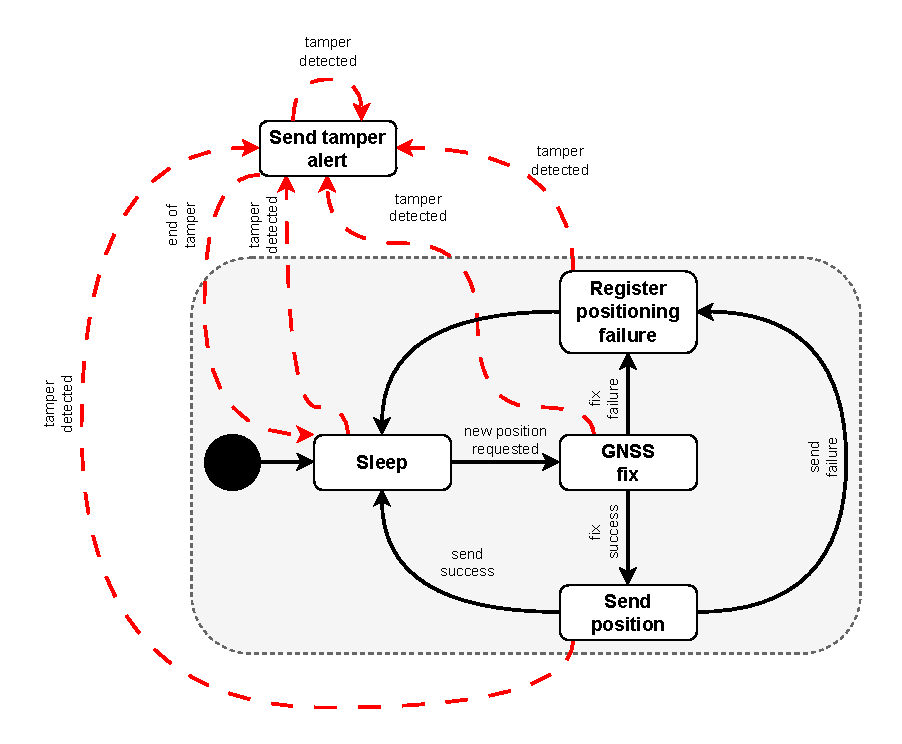
\includegraphics[width=\columnwidth]{imgs/fsm_example.pdf} % Adjust size and add filename
    \caption{Máquina de estados de uma aplicação de rastreamento.} % The visual text caption
    \label{fig:fsm_example} % The key used to reference this image in text
\end{figure}

Como exemplo didático de execução de uma \textit{Behavior Tree}, vamos considerar a aplicação de um dispositivo rastreador, conforme ilustrado na máquina de estados da figura \ref{fig:fsm_example}.
Neste primeiro momento, vamos considerar apenas a parte destacada pela área em fundo cinza. Inicialmente, o dispositivo inicia-se no estado \texttt{Sleep}, que representa um modo de baixo consumo de energia.
Quando ocorre o evento de nova aquisição de posicionamento \texttt{new position requested}, o dispositivo vai para o estado \texttt{GNSS fix} para executar a aquisição de posicionamento pelo módulo GNSS (\textit{Global Navigation Satellite System}.
Caso o \textit{fix} ocorra com sucesso, o dispositivo para vai o estado \texttt{Send position} para transmissão da nova posição geográfica, e, por fim, volta a dormir em caso de sucesso da transmissão.
Caso o dispositivo falhe na aquisição de posição pelo módulo GNSS ou na transmissão desta informação, o dispositivo vai para o estado \texttt{Register positioning failure} para registrar a ocorrência da falha e volta para o estado \texttt{Sleep}.

A \textit{Behavior Tree} que representa a modelagem da mesma aplicação citada anteriormente é apresentada na figura \ref{fig:bt_example}.
De forma semelhante, vamos considerar apenas a parte do modelo destacada pela área em fundo cinza. A execução da árvore se inicia a partir do nó \textit{Fallback} na raiz e percorre os nós da árvore executando os filhos mais à esquerda até atingir o nó de condição \textit{New position requested}. Ao ser executado, este nó de condição pode retornar \textit{Failure} ou \textit{Success}.
Caso esse nó retorne \textit{Failure}, ele retorna a execução e seu \textit{status} para o nó pai \textit{Sequence} logo acima, que avalia o valor a partir de sua função de política de controle e decide retornar para o nó pai \textit{Fallback}, atingindo a raiz da árvore.
Ao receber o \textit{status} \textit{Failure}, o nó raiz \textit{Fallback} decide executar seu próximo nó filho \textit{Sleep}.
Esta execução representa a operação em modo de baixo consumo da aplicação.
Caso a execução do nó \textit{New position requested} retorne o \textit{status} \textit{Success}, o seu nó pai \textit{Sequence} decidirá, neste momento, executar seu próximo nó filho \textit{Fallback}.
Em consequência, o \textit{tick} da árvore será propagado novamente para os nós filho à esquerda e, eventualmente, o nó \textit{GNSS fix} será atingido.
Caso seu valor de retorno seja \textit{Success}, o nó \textit{Send position} será executado. A partir da árvore é possível verificar que o nó \textit{Register positioning failure} só será executado caso o nó \textit{GNSS fix} ou \textit{Send position} retorne \textit{Failure}. Desta maneira, nota-se que a árvore executa de forma semelhante à máquina de estados apresentada na figura \ref{fig:fsm_example}. 

% 2. Insert the figure environment where you want it
\begin{figure}[ht]
    \centering % Centers the image
    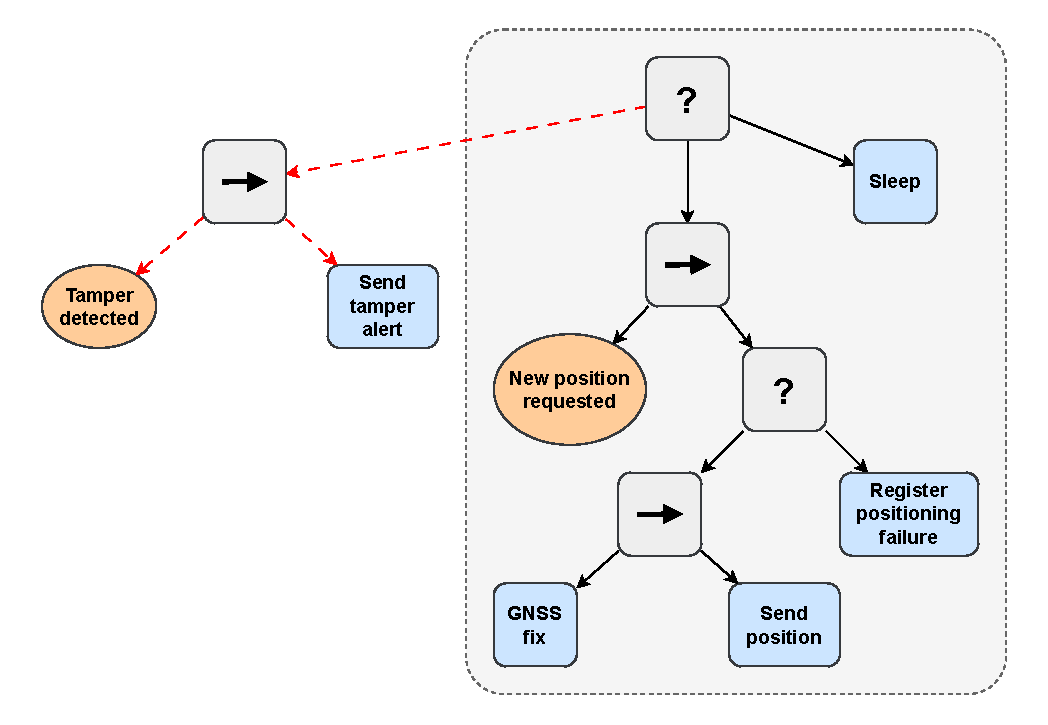
\includegraphics[width=\columnwidth]{imgs/bt_example.pdf} % Adjust size and add filename
    \caption{Exemplo de \textit{Behavior Tree} numa aplicação de rastreamento.} % The visual text caption
    \label{fig:bt_example} % The key used to reference this image in text or
\end{figure}

\subsection{Modularidade e reatividade em \textit{Behavior Trees}}

Para verificarmos o poder de abstração de uma \textit{Behavior Tree}, vamos estender a aplicação apresentada anteriormente adicionando uma nova funcionalidade que detecta quando o dispositivo rastreador é violado, representada pelo estado \texttt{Send tamper alert} e pelas transições \texttt{tamper detected}, conforme está ilustrado na figura \ref{fig:fsm_example}. Desta maneira, toda vez que o dispositivo detectar uma violação, como a abertura do seu invólucro ou caixa, ele deve enviar um alerta de violação continuamente até a indicação de violação ser interrompida. Como a detecção de violação deve operar a qualquer momento de funcionamento do dispositivo, a transição \texttt{tamper detected} deve partir de qualquer estado possível do sistema.
Assim, para realizar a funcionalidade como esperado, a adição do estado \texttt{Send tamper alert} requer a adição de mais cinco transições \texttt{tamper detected}, uma para cada estado pré-existente no modelo e outra transição com origem e destino no próprio estado \texttt{Send tamper alert}.
Por fim, a transição \texttt{end of tamper} foi adicionada de forma ilustrativa para indicar a interrupção do evento de violação e a ida para o modo de baixo consumo de energia.

Em contrapartida, a adição desta funcionalidade no modelo da \textit{Behavior Tree} requer apenas a inclusão de uma nova ramificação a partir do nó raiz \textit{Fallback}, conforme pode ser verificado na figura \ref{fig:bt_example}.
Esta nova ramificação consiste em um nó \textit{Sequence} seguido pelos nós de condição e execução, \textit{Tamper detected} e \textit{Send tamper alert}, respectivamente.
Nesta versão estendida do modelo em \textit{Behavior Tree}, observa-se uma vantagem quando comparada ao modelo de máquina de estados: a modularidade.
Enquanto a adição da nova funcionalidade resultou na adição de várias transições no modelo de máquina de estados, na \textit{Behavior Tree} apenas uma nova ramificação foi adicionada.
A alteração do modelo em máquina de estados se torna visualmente mais complexa, mas, além disso, a adição de várias transições entre os estados pré-existentes e o novo estado adicionado exige a alteração dos próprios estados em si.
Já no modelo em \textit{Behavior Tree}, a adição da nova ramificação apenas alterou o nó raiz \textit{Fallback}. 

Outra característica a ser destacada no modelo de \textit{Behavior Tree} é sua capacidade de reatividade, inerente na própria execução da árvore. Vamos considerar que o dispositivo rastreador não está em violação (o nó \textit{Tamper detected} retorna \textit{FAILURE}) e que o nó \textit{GNSS fix} está retornando o \textit{status} \textit{RUNNING}, indicando que esta ação requer um intervalo de tempo para ser concluída. Neste cenário, ao retornar \textit{RUNNING}, a árvore não avança sua execução e verifica continuamente o resultado da ação \textit{GNSS fix}, mas também verifica todos os nós à esquerda do nó em execução para avaliar se o contexto permanece o mesmo. Caso ocorra uma detecção de violação, alterando o \textit{status} do nó \textit{Tamper detected} para \textit{SUCCESS}, a árvore automaticamente começa a executar a nova ramificação habilitada (nós \textit{Sequence}, \textit{Tamper detected} e \textit{Send tamper alert}) e interrompe a execução do nó \textit{GNSS fix}. Assim, é possível verificar a reatividade natural da \textit{Behavior Tree} quando ocorre uma alteração no contexto atual de execução sem que haja a necessidade dos nós terem conhecimento desta alteração.

\section{Framework Proposto}

Como proposta deste trabalho, apresentamos o \textbf{BTreeFy}, um \textit{framework} de \textit{Behavior Tree} para Sistemas Embarcados com Recursos Restritos. O principal objetivo para o desenvolvimento deste \textit{framework} é permitir a execução de \textit{Behavior Trees} em ambientes com recursos computacionais restritos. Para este fim, o projeto deste \textit{framework} considerou princípios e características necessários para que esse objetivo fosse atingido.
As principais características do projeto deste \textit{framework} e suas justificativas são listadas a seguir:


\paragraph{\textbf{Execução iterativa}} Diferentemente de outras implementações que utilizam chamadas recursivas, nossa proposta adota uma abordagem iterativa. Em uma implementação recursiva clássica, o processador precisa empilhar o contexto em cada chamada. Em uma estrutura de árvore muito profunda, o crescimento da pilha de chamadas resultaria em um consumo imprevisível e excessivo de memória RAM, comprometendo a estabilidade em plataformas restritas.

\paragraph{\textbf{Utilização da representação LCRS plana}} Uma árvore pode ser representada de diversas maneiras na memória. Para sistemas restritos, a primeira decisão de projeto foi evitar totalmente a alocação dinâmica e os ponteiros tradicionais. O BTreeFy armazena todos os nós da árvore de forma contígua em um único \textit{array} alocado estaticamente, utilizando índices para codificar as relações de parentesco. Isso reduz drasticamente o consumo de memória por eliminar o \textit{overhead} dos ponteiros (especialmente em arquiteturas de 32 bits) e melhora a localidade de referência na \textit{cache} do processador.
A segunda decisão foi como codificar as relações dentro desse \textit{array}. Ao invés de representar explicitamente nós n-ários (que exigem estruturas de tamanho variável), adotamos a representação \textit{Left-Child Right-Sibling} (LCRS), essencialmente aplicando a Transformada de Knuth para converter a BT n-ária em uma estrutura equivalente binária. Nesta representação padronizada, cada nó armazena apenas dois índices: seu primeiro filho (filho mais à esquerda) e seu próximo irmão (à direita). Como a ordem de execução da BT é estritamente da esquerda para a direita, a estrutura LCRS mapeia com perfeição a navegação exigida durante o \textit{tick}, viabilizando uma implementação universal, leve e previsível.

\paragraph{\textbf{Implementação puramente em ANSI C}} a implementação do \textit{framework} em ANSI C e ausência de dependências externas possibilitam uma maior integração e portabilidade. Desta maneira, o \textit{framework} pode ser usado em aplicações \textit{bare metal} como também em ambientes com Sistemas Operacionais de Tempo Real como o \textit{FreeRTOS} e \textit{Zephyr RTOS}.

\paragraph{\textbf{Geração de código}} O projeto disponibiliza um utilitário que interpreta um arquivo XML (produzido por editores padrão como o \textit{Groot 2}) e gera automaticamente o código-fonte C contendo o \textit{array} estático LCRS da árvore. Pelo fato de todo o fluxo de controle e as relações hierárquicas serem codificadas estaticamente em um único \textit{array} \textit{read-only}, a geração de código da BT é direta e otimizada. Isso difere enormemente de ferramentas equivalentes de máquinas de estados, cuja tradução de grafo para código costuma demandar a geração de dezenas de funções de preempção cruzada para garantir as interrupções de estados.

\subsection{Modelagem do nó e da árvore no BTreeFy}

Na implementação do \textit{BTreeFy}, os objetos básicos são o nó e a árvore. Na definição do nó (ver listagem \ref{lst:btf_node}), o campo \texttt{status} é utilizado para armazenar o estado de execução do nó durante o processamento da árvore. Esse campo pode assumir os valores \texttt{FAILURE}, \texttt{SUCCESS} e \texttt{RUNNING}, semelhante à execução de uma \textit{Behavior Tree}. Os campos \texttt{child} e \texttt{sibling} armazenam os índices das referências dos nós filho e irmão do nó, indicando a estrutura \textit{left-child right-sibling}. A referência do nó pai através do campo \texttt{parent} é usada para navegar em direção à raiz da árvore. Na execução de uma \textit{Behavior Tree}, é necessário voltar aos nós pais após a execução de um nó para avaliar qual decisão será realizada de acordo com a política do nó de controle em questão. Por fim, o campo \texttt{handler\_fn} armazena um ponteiro para função que pode representar uma função de política de um nó de controle ou uma função de ação de um nó folha. A escolha de definir o campo \texttt{handler\_fn} como \texttt{void *} é devido à possibilidade deste campo poder receber um ponteiro para função de tipos diferentes, já que o protótipo de uma função de política é diferente do protótipo da função de uma ação, como será visto em seções adiante.

\red{Mudar o tipo do índice da árvore um tipo genérico, e acrescentar que a depender do tamanho da árvore muda o tipo. Isso faz econimizar memória }

\begin{lstlisting}[language=C, caption={Definição do objeto nó no \textit{BTreeFy}}, label={lst:btf_node}]
struct btf_node
{
    enum btf_node_status status;
    uint32_t             parent;
    uint32_t             child;
    uint32_t             sibling;
    void                 *handler_fn;
};
\end{lstlisting}

A definição da definição da árvore no \textbf{BTreeFy} é apresentada na listagem \ref{lst:btf_tree}. O campo \texttt{nodes} armazena o \textit{array} de nós da árvore e o campo \texttt{size} indica a quantidade de nós deste \textit{array}, e consequentemente, o tamanho da árvore. Também, a árvore pode armazenar um dado do usuário através do ponteiro no campo \texttt{data} e seu tamanho em \texttt{datalen}. Este dado de usuário associado à árvore pode ser acessado nas funções de ação dos nós folha implementadas pelo usuário, permitindo que os nós troquem dados entre si. Por fim, o campo \texttt{running\_node\_index} armazena o índice do nó que está em execução ou estado de \texttt{RUNNING} no momento. É através desta referência que o \texttt{framework} consegue abortar um nó em execução, caso a ramificação da árvore na qual ele se encontra não seja mais alcançável na execução atual.

É importante notar que, embora o exemplo na Listagem \ref{lst:btf_tree} utilize \texttt{uint32\_t} para máxima compatibilidade, na prática, para aplicações embarcadas típicas (onde a BT não ultrapassa algumas centenas de nós), esses índices e tamanhos podem ser perfeitamente reduzidos para tipos \texttt{uint8\_t} ou \texttt{uint16\_t}. Em um cenário de máxima otimização com \texttt{uint8\_t} (limite de 255 nós), a economia de memória RAM é expressiva, reduzindo o custo por nó drasticamente.

\begin{lstlisting}[language=C, caption={Definição do objeto árvore no \textit{BTreeFy}}, label={lst:btf_tree}]
struct btf_tree
{
    struct btf_node *nodes;
    uint32_t         size;
    void *           data;
    size_t           datalen;
    uint32_t         running_node_index;
};
\end{lstlisting}

 

\section{Estudo de caso}

Devido à falta de consenso na literatura atual sobre metodologias unificadas de avaliação de \textit{Behavior Trees} \cite{gugliermo_evaluating_2024}, nesta seção é apresentado um estudo de caso com métricas próprias, com o intuito de demonstrar a aplicabilidade do \textit{framework} BTreeFy em um sistema embarcado. O cenário de uso consiste em uma aplicação de rastreamento de ativos, cujos modelos conceituais para FSM e BT foram introduzidos nas Figuras \ref{fig:fsm_example} e \ref{fig:bt_example}, respectivamente. O objetivo primário é quantificar os ganhos de modularidade e flexibilidade promovidos pelas BTs e medir o impacto de desempenho e consumo de recursos. Como referência, desenvolvemos a mesma aplicação utilizando o Zephyr State Machine Framework (SMF). Ambas as abordagens foram implementadas sobre o Zephyr RTOS e avaliadas sob duas variantes: uma versão base (rastreamento de posição) e uma versão estendida com funcionalidade de detecção de violação (\textit{tamper}), permitindo analisar o esforço de extensão de código de ambas as abordagens.

\subsection{Configuração do Experimento}
Para a avaliação das restrições de tempo real, a aplicação de estresse foi embarcada em um microcontrolador STM32 Nucleo-F091RC (ARM Cortex-M0, 256 KB Flash, 32 KB RAM). Os testes de memória e equivalência comportamental foram realizados utilizando o ambiente nativo \textit{native\_sim} do Zephyr. O \textit{framework} Zbus, componente do Zephyr RTOS para barramento assíncrono, foi adotado para abstrair os módulos de \textit{hardware}. Nas BTs, a execução da árvore é ativada através de \textit{ticks} emitidos sempre que um novo evento (como recepção GNSS ou rádio) é publicado no Zbus, caracterizando uma arquitetura orientada a eventos que otimiza recursos computacionais ao evitar \textit{polling} contínuo \cite{wu_microsbt_2021}.

\subsection{Resultados e Discussão}
A avaliação foi baseada em cinco eixos distintos, e a síntese dos resultados é apresentada na Tabela \ref{tab:results_summary}.

\begin{table}[ht]
\centering
\caption{Síntese dos resultados da avaliação entre BT e FSM}
\label{tab:results_summary}
\begin{tabular}{lrr}
\hline
\textbf{Métrica} & \textbf{BT (BTreeFy)} & \textbf{FSM (Zephyr SMF)} \\
\hline
Linhas de código (\textit{tamper}) & \textbf{12} & 30 \\
Acréscimo de Flash (\textit{tamper}) & 224 B & 224 B \\
Footprint RAM (motor base) & $\sim$32 B & $\sim$20 B \\
Footprint Flash (motor base) & $\sim$866 B & $\sim$768 B \\
Latência média (Cortex-M0) & 43,00 $\mu$s & \textbf{3,73 $\mu$s} \\
Equivalência comportamental & Aprovado & Aprovado \\
\hline
\end{tabular}
\end{table}

\paragraph{\textbf{Modificabilidade e Modularidade}} 
A vantagem da BT torna-se evidente na extensão da aplicação para incluir a detecção de violação. A implementação em BT exigiu 2,5$\times$ menos código condicional que a FSM (12 linhas de código em comparação com as 30 linhas necessárias para a FSM). Enquanto a FSM obriga o programador a inserir blocos condicionais de transição de preempção em quase todos os estados existentes, a modificação na BT concentrou-se apenas na adição de uma ramificação independente na raiz, demonstrando excelente separação de interesses e corroborando evidências empíricas de que BTs facilitam modificações e reuso de comportamentos \cite{dragule_effects_2025}.

\paragraph{\textbf{Consumo de Recursos (Footprint)}} 
Ambas as abordagens adicionaram exatos 224 bytes de Flash para incluir a funcionalidade de violação, demonstrando um custo marginal equivalente. A BT apresenta um pequeno custo fixo pelo uso do seu motor de execução em comparação à FSM, adicionando cerca de 1 KB em Flash e 32 bytes em RAM. Para aplicações embarcadas modernas, esse custo estático é negligenciável diante do benefício arquitetural.

\paragraph{\textbf{Desempenho de Execução (Latência)}}
Para a medição de latência temporal, foi gerado proceduralmente um modelo de decisão estressante e profundo com 125 nós lógicos. A execução completa na BT registrou um tempo médio de 43 $\mu$s. Embora a FSM convencional execute de maneira consideravelmente mais rápida (cerca de 3,7 $\mu$s), o custo de processamento da BT permanece na ordem de algumas dezenas de microssegundos, suportando folgadamente requisitos de tempo-real de sistemas cujas reações situam-se na faixa de milissegundos.

\paragraph{\textbf{Equivalência Comportamental}} 
Ambas as aplicações foram testadas sob as mesmas sequências pseudo-aleatórias intensivas de eventos de sensores. Demonstrou-se, com zero divergências na emissão de comandos para os atuadores, que a abordagem baseada em \textit{Behavior Trees} exibe um rigoroso determinismo, sendo comportamentalmente idêntica à já consolidada máquina de estados do Zephyr.

\section{Conclusão}

Este artigo apresentou o BTreeFy, um \textit{framework} projetado desde o princípio para transpor a lacuna arquitetural e metodológica que impedia o uso prático de \textit{Behavior Trees} em Sistemas Embarcados com Recursos Restritos. Através de decisões como a execução iterativa da travessia da árvore e o uso da representação estática de memória baseada em índices e estruturas \textit{Left-Child Right-Sibling}, demonstramos que é possível obter os mesmos benefícios arquiteturais das BTs presentes em domínios avançados (como Robótica e IA) em microcontroladores \textit{bare-metal} com rígidas limitações de RAM e Flash.

O estudo de caso realizado, uma aplicação de rastreamento de ativos sobre o Zephyr RTOS, evidenciou quantitativamente as vantagens e \textit{trade-offs} envolvidos. Ao adicionar a funcionalidade preemptiva de detecção de violação (\textit{tamper}), a BT revelou seu poder de modularidade: demandou 2,5 vezes menos alterações no código C em relação à clássica Máquina de Estados (FSM), visto que novos comportamentos são orquestrados no modelo (a árvore XML) sem infectar as funções e guardas já existentes. 

Avaliamos rigorosamente os custos que acompanham esse ganho de abstração. Em termos de uso estático de memória (\textit{footprint}), o \textit{framework} impõe uma modesta "taxa base" de cerca de 1 KB em Flash e algumas dezenas de bytes em RAM, valor este consideravelmente pequeno face à capacidade da maioria das plataformas de IoT modernas (como a família Cortex-M). No quesito temporal, embora as BTs possuam um \textit{overhead} natural de execução devido à navegação hierárquica e ao mecanismo de \textit{ticks} iterativos, a medição em \textit{hardware} indicou uma latência máxima de cerca de 43 $\mu$s para uma decisão complexa (uma árvore estressada com mais de 100 nós lógicos). Esse tempo atende de modo satisfatório os requisitos operacionais da ampla maioria das aplicações práticas, cujas frequências de eventos estão tipicamente concentradas na faixa dos milissegundos.

Em suma, as \textit{Behavior Trees} confirmam-se não apenas como uma alternativa viável, mas, em muitos casos de sistemas de controle com regras de negócios evolutivas, como uma arquitetura superior às tradicionais Máquinas de Estados. Como trabalhos futuros, planejamos conduzir avaliações com outros escalonadores em sistemas embarcados e implementar suporte integrado a mecanismos de sincronização para nós concorrentes (como os do tipo \textit{Parallel}), a fim de evitar condições de corrida de forma estruturada e previsível \cite{colledanchise_handling_2022}, expandindo ainda mais as classes de problemas resolvidas pelo BTreeFy.

\bibliographystyle{IEEEtran}
\bibliography{sbesc26-refs}

\end{document}
